\documentclass[tikz,border=8pt]{standalone}
\usepackage{amsmath,amssymb}
\usetikzlibrary{arrows.meta,automata,positioning,quotes}
\begin{document}
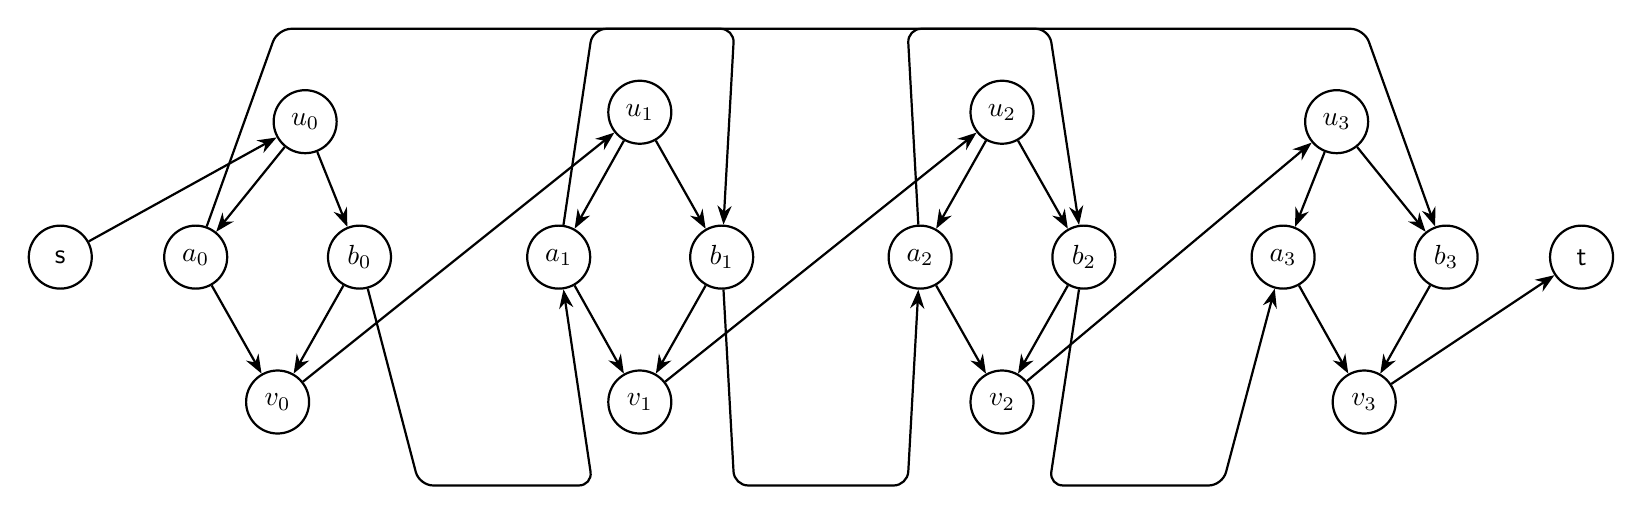
\begin{tikzpicture}[x=1cm,y=1cm]
\tikzset{
  graphnode/.style={circle,draw,thick,minimum size=8mm,inner sep=1pt,font=\sffamily},
  directed/.style={-{Stealth[length=2.4mm]},thick},
  undirected/.style={thick}
}
\node[graphnode] (n_s) at (-3.66,0.00) {s};
\node[graphnode] (n_t) at (15.66,0.00) {t};
\node[graphnode] (n_u_0) at (-0.55,1.72) {$u_{0}$};
\node[graphnode] (n_v_0) at (-0.90,-1.84) {$v_{0}$};
\node[graphnode] (n_a_0) at (-1.94,0.00) {$a_{0}$};
\node[graphnode] (n_b_0) at (0.14,0.00) {$b_{0}$};
\node[graphnode] (n_u_1) at (3.70,1.84) {$u_{1}$};
\node[graphnode] (n_v_1) at (3.70,-1.84) {$v_{1}$};
\node[graphnode] (n_a_1) at (2.67,0.00) {$a_{1}$};
\node[graphnode] (n_b_1) at (4.74,0.00) {$b_{1}$};
\node[graphnode] (n_u_2) at (8.30,1.84) {$u_{2}$};
\node[graphnode] (n_v_2) at (8.30,-1.84) {$v_{2}$};
\node[graphnode] (n_a_2) at (7.26,0.00) {$a_{2}$};
\node[graphnode] (n_b_2) at (9.34,0.00) {$b_{2}$};
\node[graphnode] (n_u_3) at (12.55,1.72) {$u_{3}$};
\node[graphnode] (n_v_3) at (12.90,-1.84) {$v_{3}$};
\node[graphnode] (n_a_3) at (11.87,0.00) {$a_{3}$};
\node[graphnode] (n_b_3) at (13.94,0.00) {$b_{3}$};
\draw[directed] (n_u_0) -- (n_a_0);
\draw[directed] (n_u_0) -- (n_b_0);
\draw[directed] (n_a_0) -- (n_v_0);
\draw[directed] (n_b_0) -- (n_v_0);
\draw[directed] (n_u_1) -- (n_a_1);
\draw[directed] (n_u_1) -- (n_b_1);
\draw[directed] (n_a_1) -- (n_v_1);
\draw[directed] (n_b_1) -- (n_v_1);
\draw[directed] (n_u_2) -- (n_a_2);
\draw[directed] (n_u_2) -- (n_b_2);
\draw[directed] (n_a_2) -- (n_v_2);
\draw[directed] (n_b_2) -- (n_v_2);
\draw[directed] (n_u_3) -- (n_a_3);
\draw[directed] (n_u_3) -- (n_b_3);
\draw[directed] (n_a_3) -- (n_v_3);
\draw[directed] (n_b_3) -- (n_v_3);
\draw[directed] (n_s) -- (n_u_0);
\draw[directed] (n_v_0) -- (n_u_1);
\draw[directed] (n_v_1) -- (n_u_2);
\draw[directed] (n_v_2) -- (n_u_3);
\draw[directed] (n_v_3) -- (n_t);
\draw[directed,rounded corners=5pt] (n_a_0) -- (-0.90,2.90) -- (4.90,2.90) -- (n_b_1);
\draw[directed,rounded corners=5pt] (n_b_0) -- (0.90,-2.90) -- (3.10,-2.90) -- (n_a_1);
\draw[directed,rounded corners=5pt] (n_a_1) -- (3.10,2.90) -- (8.90,2.90) -- (n_b_2);
\draw[directed,rounded corners=5pt] (n_b_1) -- (4.90,-2.90) -- (7.10,-2.90) -- (n_a_2);
\draw[directed,rounded corners=5pt] (n_a_2) -- (7.10,2.90) -- (12.90,2.90) -- (n_b_3);
\draw[directed,rounded corners=5pt] (n_b_2) -- (8.90,-2.90) -- (11.10,-2.90) -- (n_a_3);
\end{tikzpicture}
\end{document}
